%=========================================================

% Here you can choose to compile with or without solutions.
% However, this definition is ignored if you use any
% command from the `Makefile`.
\providecommand{\withSol}{\iftrue}

%=========================================================

\documentclass
[twoside,english,colorbacktitle,accentcolor=tud9c]
{tudexercise}

\usepackage[T1]{fontenc}
\usepackage[latin9]{inputenc}
\usepackage{float}
\usepackage{listings}
\usepackage{amstext}
\usepackage{amsmath}
\usepackage{graphicx}
\usepackage{setspace}
\usepackage{multicol}
\usepackage{mathtools}
\usepackage{dsfont}
\usepackage{units}
\usepackage{subfigure}
\usepackage{color}
\usepackage{booktabs}
\usepackage{fancyref}
\usepackage[ngerman,english]{babel}

%=========================================================

\def\homework{4}
\def\homeworkVer{1}
\def\homeworkSolVer{1}
\def\lecture{Machine Learning}
\def\semester{Summer Semester 2019}
\def\prof{Prof. Dr. J. Peters, H. Abdulsamad, S. Stark, D.Koert}
\def\deadline{Due date: Friday, 19 Juli 2019 (17:00)\\
You need to hand in the pdf in moodle \textbf{and} a printed version to the postbox from the IAS secretary office (S2 02 | E315)}

%=========================================================

\ifcsname withSol\endcsname\else
  \expandafter\let\csname withSol\expandafter\endcsname
                  \csname iffalse\endcsname
\fi

\withSol
	\usepackage[solutions]{iasHomework}
\else
	\usepackage{iasHomework}
\fi

%=========================================================

% USE YOUR NAMES!
\newcommand{\studentdata}{}
%\newcommand{\studentdata}{John Doe, 1234567 \qquad Jane Doe, 7654321}

\begin{document}

	\hwtitle{}
	\maketitle
	
	\begin{examheader}
		\normalsize
		\vspace{-1em}
		Name, Surname, ID Number \hfill \studentdata{}
		\vspace{-1em}
	\end{examheader} 
	
	\textbf{Name, Surname, ID Number \hfill \studentdata{}}
	
	\newif\ifvimbug
\vimbugfalse

\ifvimbug
\begin{document}
\fi

\exercise{Support Vector Machines}
In this exercise, you will use the dataset \texttt{iris-pca.txt}. It is the same dataset used for Homework 3, but the data has been pre-processed with PCA and only two kinds of flower (`Setosa' and `Virginica') have been kept, along with their two principal components. Each row contains a sample while the last attribute is the label ($0$ means that the sample comes from a `Setosa' plant, $2$ from `Virginica').
\\You are allowed to \texttt{numpy} functions (e.g., \texttt{numpy.linalg.eig}). For quadratic programming we suggest \texttt{cvxopt}.
\begin{questions}

%----------------------------------------------

\begin{question}{Definition}{3}
Briefly describe SVMs. What is their advantage w.r.t. other linear approaches we discussed this semester? 

\begin{answer}
A Support Vector Machine (SVM) is a non-probabilistic discriminative classifier, which is defined by two hyperplanes that define the class borders, and a margin in between of these hyperplanes. The hyperplane in between of the two class hyperplanes is the maximum-margin hyperplane. An SVM model is a representation of the labeled examples in points in space, mapped in such a way, that the examples of the separated classes are divided by a margin, which is as wide as possible. If no slack variables are included, the algorithm does not allow for any points to lie within the margin. The points, that lie at the border of the margin, and thus define it, are called support vectors. New examples are mapped into the same space and their class label is predicted to belong to a category based on the side of the margin, on which they are located.
In comparison to other linear approchases, SVMs can also do complex, non-linear classification by employing the kernel trick. Kernel can implicitly map inputs into high-dimensional feature spaces. Unlike other methods, SVMs work well with unstructured data like text, images or trees. Furthermore we do not need many prior knowledge or assumptions on the data, as in the case of LDA with a Bayes Classifier.
Furthermore, SVMs are an approximate imlementation of the structural risk minimization principle. If the data is linearly separable, the empirical risk of SVM classifiers is zero. It follows, that the risk bound will be approximately minimized. SVMs thus have a bulit-in generalization ability.
\end{answer}
\end{question}

%----------------------------------------------

\begin{question}{Quadratic Programming}{2}
Formalize SVMs as a constrained optimization problem.
\begin{answer}
Assuming linearly separable data, SVMs can be formalized as constrained optimization problem as follows
 (see lecture notes of Andrew Ng):
\begin{equation}
\begin{aligned} \min _{w, b} & \frac{1}{2}\|w\|^{2} \\ \text { s.t. } & y^{(i)}(w^{T} x^{(i)}+b) \geq 1, \quad i=1, \ldots, m \end{aligned}
\end{equation}
$\mathbf{x}_{i} \in \mathbb{R}^{d}$ are the data points and $y_{i} \in\{-1,1\}$ the belonging class labels. Hyperplanes, that can separate the data, have the general form $y(\mathbf{x})=\mathbf{w}^{\top} \mathbf{x}+b$. The above constrained optimization problem is aiming to find the hyperplane, so that the data is linearly separated and the margin between the classes is maximized. Maximizing the margin 1$/\|\mathbf{w}\|$ is equivalent to minimizing $\frac{1}{2}\|\mathbf{w}\|^{2}$ and the constraint $y_{i}(\mathbf{w}^{\top} \mathbf{x}_{i}+b)=1$ enforces, that at least one point, a so called support vector, is on each hyperplane, that define the classes.
\end{answer}
\end{question}

%----------------------------------------------

\begin{question}{Slack Variables}{2}
Explain the concept behind slack variables and reformulate the optimization problem accordingly. 
\begin{answer}
Slack variables ``soften'' the hard constraint, that no points are allowed within the class separating margin. Now points are allowed to lie within, but this is penalized. The arguing behind this is, that SVM without using the kernel trick, can now deal with classes, that are ``overlapping'' and thus are not linearly separable. Slack variables measure the error induced by points within the margin and penalize it. This enlarges the cases, where SVM can be used for classifying. The weight $C$ allows to specify a trade-off. and the slack variables are denoted by $\xi_{i}$. This lead to the following formulation:
\begin{equation}
\begin{array}{c}{\arg \min _{\mathbf{w}, b} \frac{1}{2}\|\mathbf{w}\|^{2}+C \sum_{i=1}^{N} \xi_{i}} \\ {\textrm { s.t. } y_{i}(\mathbf{w}^{\top} \mathbf{x}_{i}+b)-1+\xi_{i} \geq 0} \\ {\xi_{i} \geq 0}\end{array}
\end{equation}
\end{answer}
\end{question}


%----------------------------------------------

%\begin{question}{Slack Variables}{7}
%Solve the optimization problem of the previous question. Show all the intermediate steps and write down the final solution.
%
\begin{answer}\end{answer}
%\end{question}


\begin{question}{The Dual Problem}{4}
What are the advantages of solving the dual instead of the primal?
	
\begin{answer}
The dual form is given by:
\begin{equation}
\begin{array}{l}{\min \sum_{i=1}^{N} \alpha_{i}-\frac{1}{2} \sum_{i=1}^{N} \sum_{j=1}^{N} \alpha_{i} \alpha_{j} y_{i} y_{j}(\mathbf{x}_{j}^{\top} \mathbf{x}_{i})} \\ {\textrm { s.t. } \alpha_{i} \geq 0} \\ {\quad \sum_{i=1}^{N} \alpha_{i} y_{i}=0}
\end{array}
\end{equation}
Exactly as the primal formulation, this is still a quadratic programming problem.
But if we now employ the nonlinear transformation $\Phi$ of the data, we can obtain a nonlinea r classifier. The new Lagrangian is:
\begin{equation}
\tilde{L}(\alpha)=\sum_{i=1}^{N} \alpha_{i}-\frac{1}{2} \sum_{i=1}^{N} \sum_{j=1}^{N} \alpha_{i} \alpha_{j} y_{i} y_{i}(\phi(\mathbf{x}_{j})^{\top} \phi(\mathbf{x}_{i}))
\end{equation}
$\Phi$  only appears in scalar products with other $\Phi$. We only need to evaluate these scalar products. The discriminant funciton can also be written with scalar products of the nonlinear features only:
\begin{equation}
y(\mathbf{x})=\sum_{i=1}^{N_{S}} \alpha_{i} y_{i} \phi(\mathbf{x}_{i})^{\top} \phi(\mathbf{x})+b
\end{equation}
This enables the kernel trick, which we talk about in the next task.
\end{answer}
\end{question}

%----------------------------------------------

\begin{question}{Kernel Trick}{3}
Explain the kernel trick and why it is particularly convenient in SVMs.
\begin{answer}
In the Kernel trick we replace every occurence of a scalar product between features with a Kerlen function.
\begin{equation}
K(\mathbf{x}_{i}, \mathbf{x}_{j})=\phi(\mathbf{x}_{i})^{\top} \phi(\mathbf{x}_{j})
\end{equation}
If we find a kernel funciton, which is equivalent to this scalar product, we can avoid mapping into a high dimensional space and instead compute the scalar-product directly.
We now can easily map the classification problem in a higher dimensional space, where any not linearly separable problem gets linearly separable.
Using this trick, SVM can classify even highly non linearly separable problems.
\end{answer}
\end{question}

%----------------------------------------------

\begin{question}[bonus]{Implementation}{5}
Implement and learn an SVM to classify the data in \texttt{iris-pca.txt}. Choose your kernel. Create a plot showing the data, the support vectors and the decision boundary. Show also the misclassified samples. Attach a snippet of your code.

\begin{answer}\end{answer}

\end{question}

\end{questions}

	
	\newif\ifvimbug
\vimbugfalse

\ifvimbug
\begin{document}
\fi

\exercise{Neural Networks}
In this exercise, you will use the dataset \texttt{mnist\_small}, divided into four files. The \textit{mnist} dataset is widely used as benchmark for classification algorithms. It contains 28x28 images of handwritten digits (pairs \texttt{<input, output>} correspond to \texttt{<pixels, digit>}).

\begin{questions}

%----------------------------------------------

\begin{question}{Multi-layer Perceptron}{20}
Implement a neural network and train it using backpropagation on the provided dataset. Choose your loss and activation functions and your hyperparameters (number of layers, neurons, learning rate, ...), briefly explaining your choices. You \textbf{cannot} use any library beside \texttt{numpy}! That is, you have to implement by yourself the loss and activation functions, the backpropagation algorithm and the gradient descent optimizer (if you want to use any).

Show how the misclassification error (in percentage) on the testing set evolves during the learning. An acceptable solution achieves an error of 8\% or less. Attach snippets of your code. 

Hint: if your network does not learn, check how the network parameters change and plot the trend of your loss function.

\begin{answer}
For the activation function I chose the sigmoid activation function. I choosed this activation function, since its derivation can be formulated using the actual function. This makes implementing gradient descent very easy. However since I choose this approach, it is non-trivial to change the activation function, since its derivative is hardcoded in the gradient descent algorithm. 

For the loss function I simply try to minimize between the output of the neural network and the label. For this purpose a one-hot-encoding is used. 

For the number of layers I went with a single layer. One layer should be sufficient enough to achieve the given metric. It is also easy to train and easy to implement. 

The number of neurons, learning rate and epoch count are chosen after my feeling of what could potentially work. 

If we now have a look at the graph showing the error on the validation set, we can see that it decreases with each epoch and reaches a minimum at 5.38 percent \ref{fig:nn}. 
\end{answer}
\begin{figure}[H]
	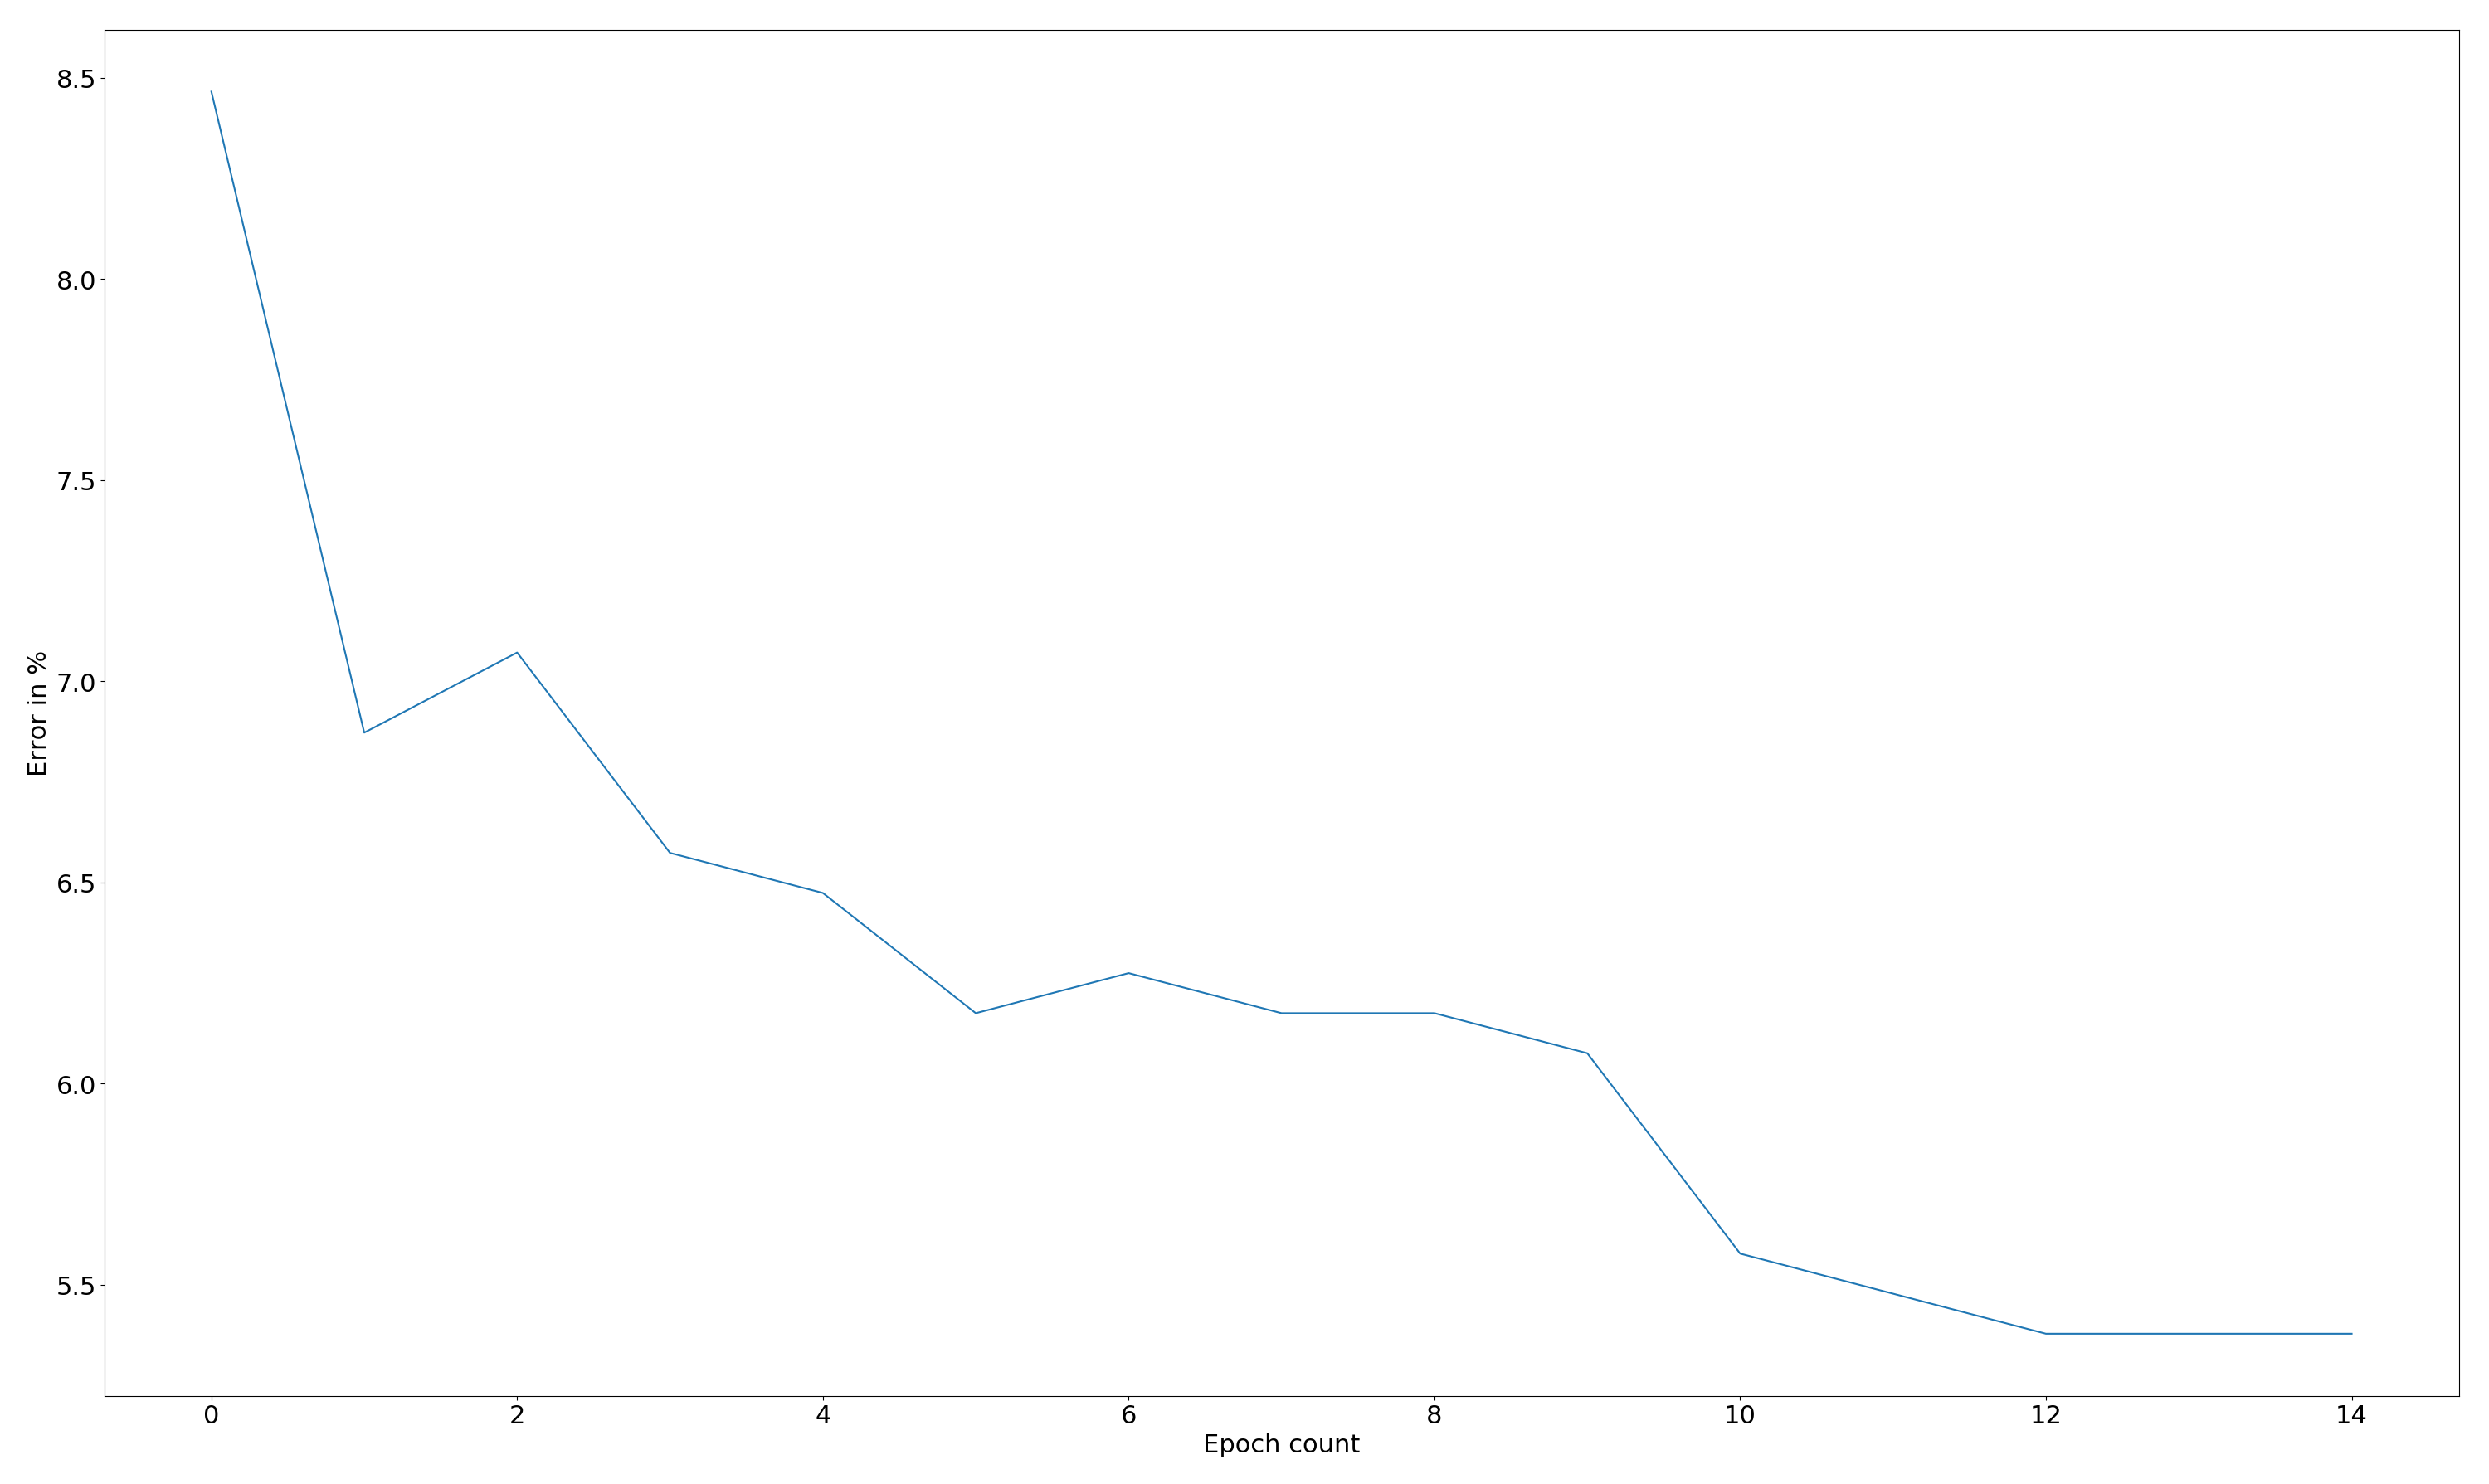
\includegraphics[width=0.8\linewidth]{pictures/NN_loss.png}
	\centering
	\caption{Classification error of the Neural Network for each epoch.}
	\label{fig:nn}
\end{figure}

Since I have already written a Neural Network last year, the code is mostly reused from that time, with removed scipy dependencies. I learned about Neuronal Networks from Tariq Rashid, so parts of my codes will borrow from his implementation. I also had some problems loading the train/test-in data with numpy, so I put them in excel and saved them again as csv, which made them work. Since this mnist dataset is sorted we need to shuffle them. I found a nice numpy function on stackoverflow which does exactly that. 
\lstinputlisting[language=Python]{code/Neural_Network.py}
\end{question}

%----------------------------------------------

\begin{question}[bonus]{Deep Learning}{5}
In recent years, deep neural networks have become one of the most used tools in machine learning. 
Highlight the qualitative differences between classical neural networks and deep networks. Which limitations of classical NN does deep learning overcome?
Give an intuition of the innovations introduced in deep learning compared to traditional NN.
(Hint: Have a look \href{http://arxiv.org/abs/1206.5538}{at this paper}. Use Google Scholar to read other scientific papers for more insights.)

\begin{answer}
The main qualitative difference between classical neural networks and deep networks is the number of layers used. Classical neural networks mostly used only a single layer. This was due to the fact that training deeper structures was hard because of vanishing gradients and considered uncesseray since the universal approximation theorem states that a single hidden layer is enough. This in combination with less training data and avaiable gpu power led to only focus on training single layer neuronal networks. 

One of the main pitfalls of classical neuronal networks was not thinking about the futher consequences of the universal approximation theorem. As it turns out, even if a single layer neural network can learn every function, the theorem doesn't state the complexity needed thus resulting in massive overfitting. 

When talking about learning representations in machine learning one key aspect is the hierachical organization of explanatory features. This means that concepts can can be defined in terms of other concepts which are all placed in a hierarchy. The more abstract, non-linear concepcts are at the top of the hierarchy. This allows Deep neural network to build more abstract features in the high levels on top of other features. In a sense a deep neural network is nothing more than a giant feature building machine. 

Another strong point for the neural network is that it allows for the re-use of features. This property exists thanks to an exponential grow in the number of paths in the circuit that arise in deeper models. 


\end{answer}

\end{question}

%----------------------------------------------

\end{questions}

	
	\newif\ifvimbug
\vimbugfalse

\ifvimbug
\begin{document}
\fi

\exercise{Gaussian Processes}
\begin{questions}

%----------------------------------------------

\begin{question}{GP Regression}{10}
Implement a Gaussian Process to fit the target function $y = \sin(x) + \sin^2(x)$ with $x \in [0, 0.005, 0.01, 0.015, \ldots, 2\pi]$. Use a squared exponential kernel, an initial mean of 0 and assume a noise variance of 0.001. Begin with no target data points and, at each iteration, sample a new point from the target function according to the uncertainty of your GP (that is, sample the point where the uncertainty is the highest) and update it. Plot your GP (mean and two times standard deviation) after iterations 1, 2, 4, 8 and 16.
In each figure, plot also the true function as ground truth and add a new marker for each new sampled point. Attach a snippet of your code.

\begin{answer}
The following pictures demonstrate our results with implementing the Gaussian Process and trying to fit the given target function. We shall notice that Gaussian Processes are a non-parametric model, meaning that they have an infinite number of parameters or that the data is our parameter. This means, that a Gaussian Process will always have a maximum uncercainity at the point where we have the least amount of data. Since the numpy linspace function spaces data points evenly out, we just need to increase the amount of points that we want to generate points which are at the maximum uncertainity of the Gaussian Process, no futher calculations required. 

I want also point out that its not a good idea to naively invert the Kernel-Matrix in order to calculate the mean. Instead we need to solve two different sets of linear equation systems. In this deparment our code borrows from Nando de Freitas (Professor at UBC) who has a fantastic lecture on Youtube, talking about the numerical problems in Gaussian Processes.
\end{answer}

Lets take a look at this beautfiul graph \ref{fig:GP_all} showing all 16 iterations of the Gaussian Process. We can see that our how the standard derivation continously shrinkes when increasing the number of training points. 
\begin{figure}[H]
	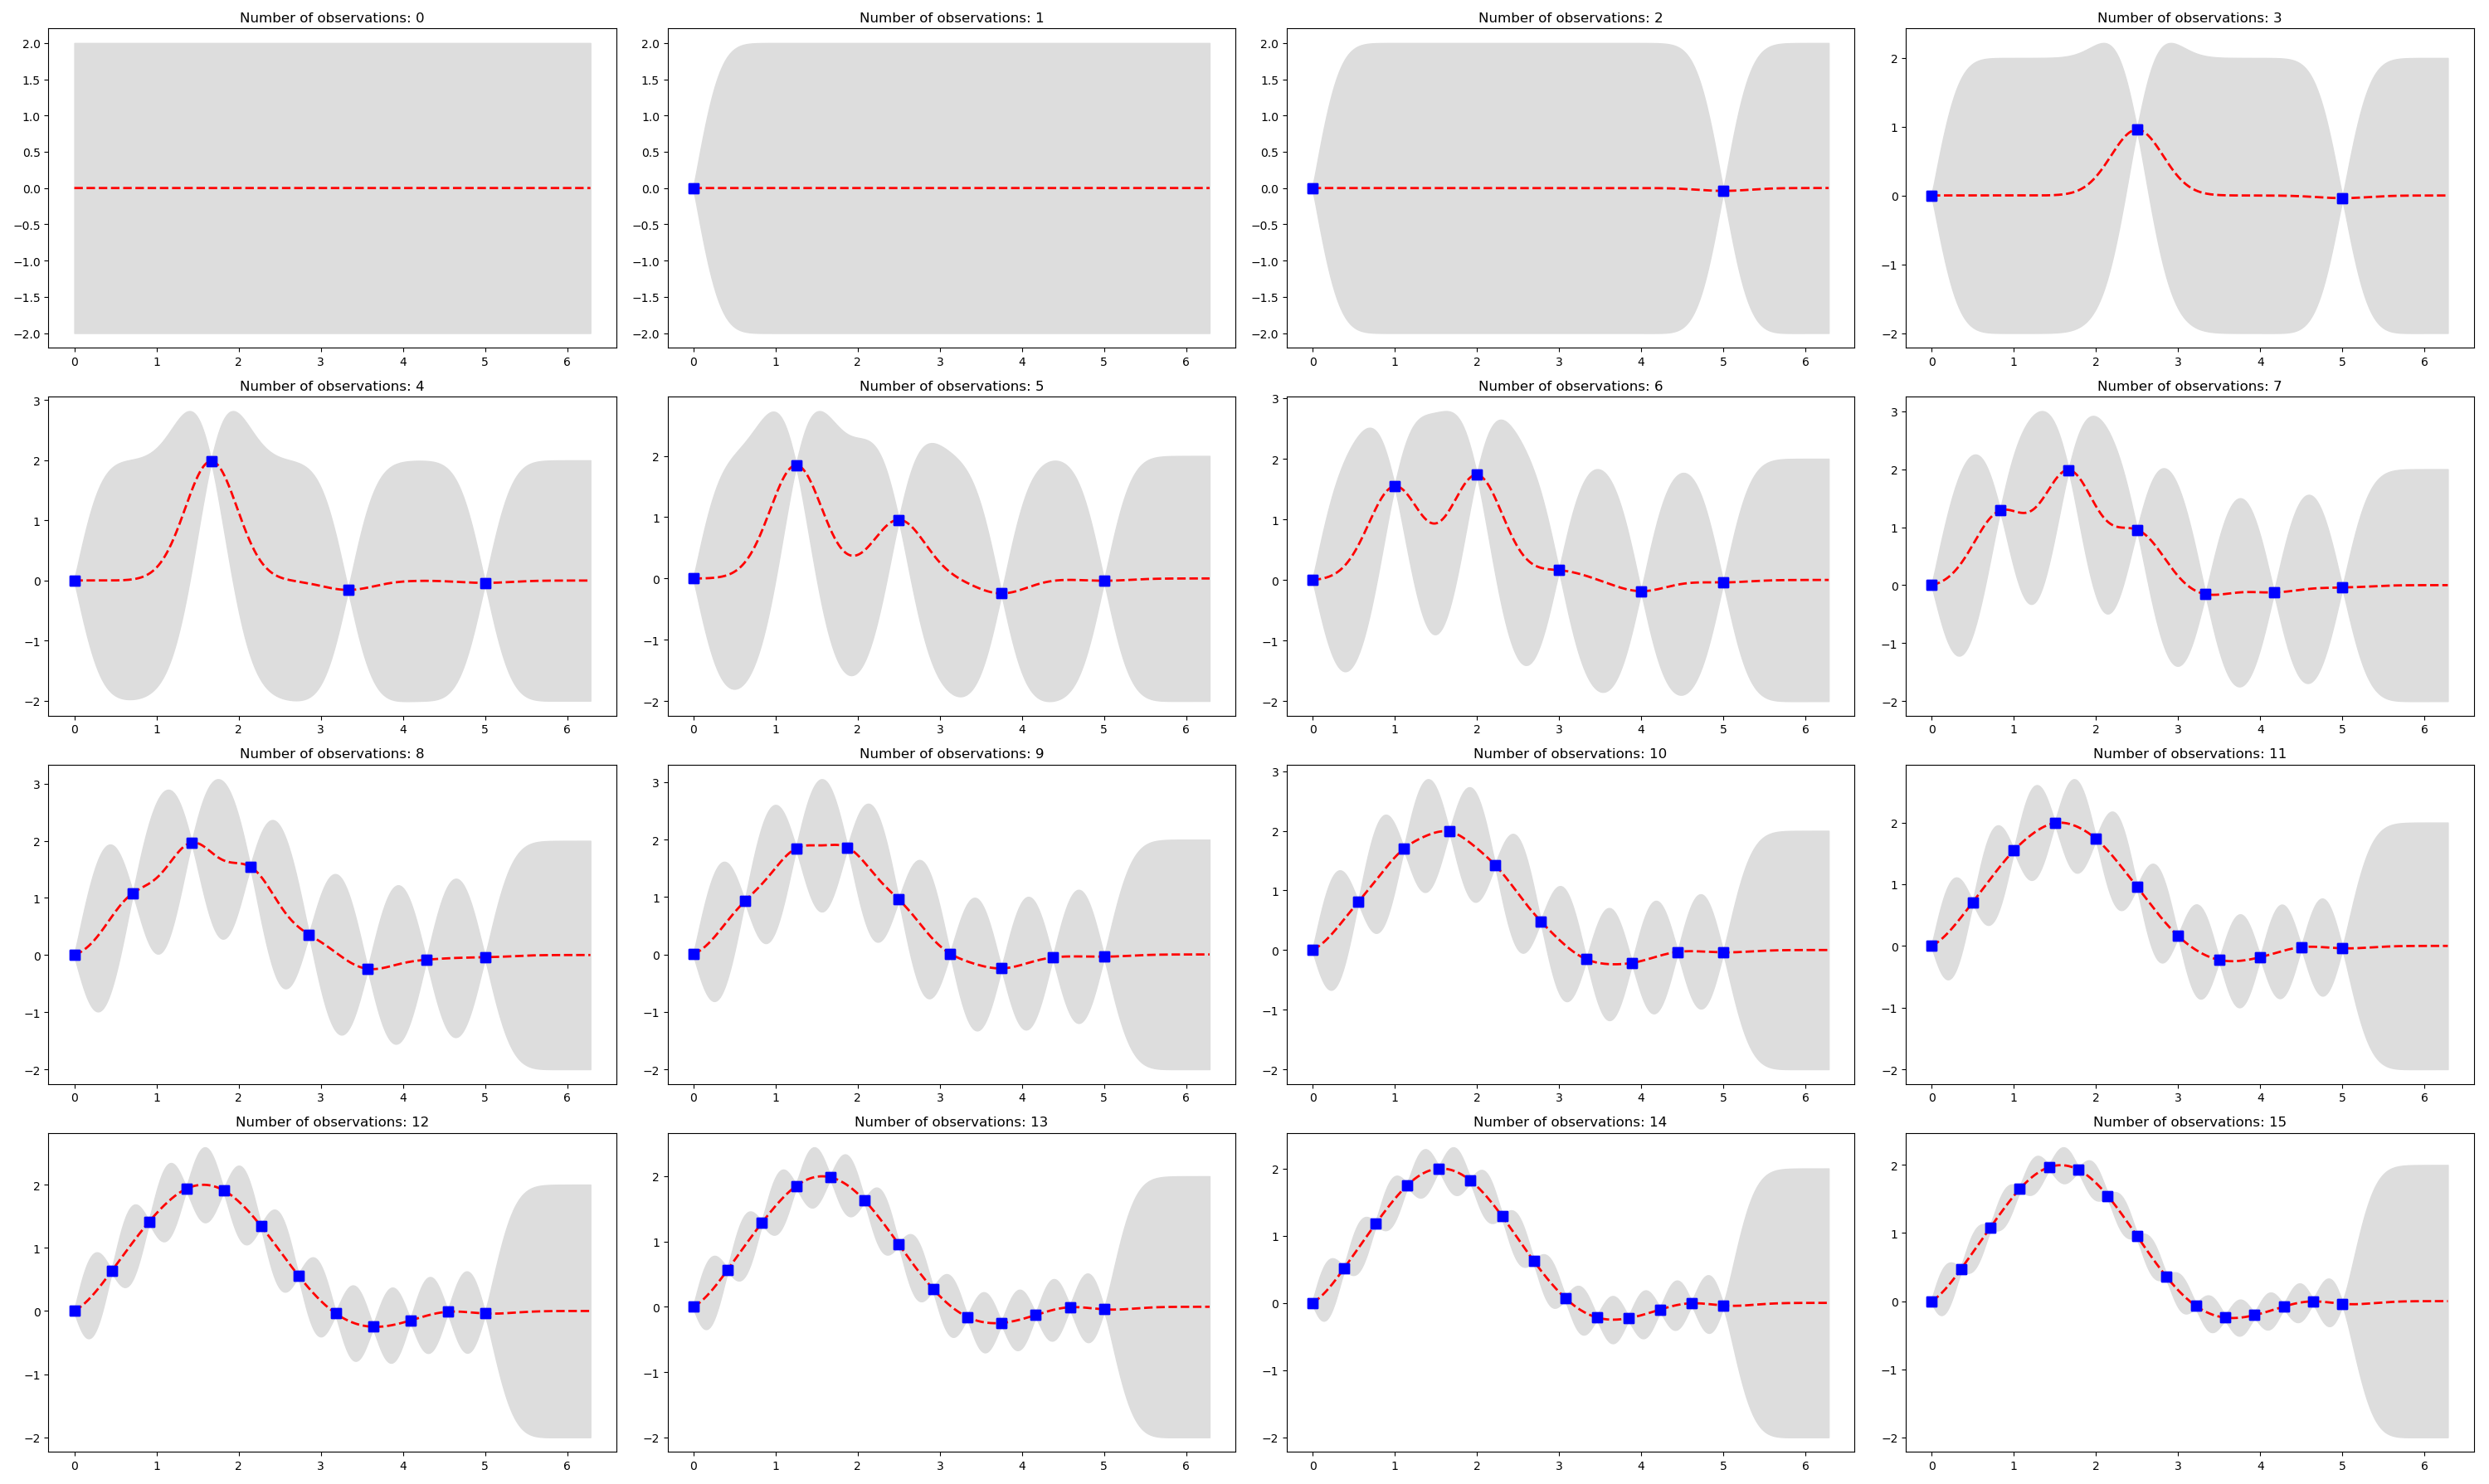
\includegraphics[width=1.0\linewidth]{pictures/GP_all_plots.png}
	\centering
	\caption{An overview of all 16 iterations for the Gaussian Process. It's beautfiul isn't it?}
	\label{fig:GP_all}
\end{figure}

In case you're overwelmed by the information density of this graph, here are the extracted versions for first \ref{fig:GP_1}, second \ref{fig:GP_2}, fourth \ref{fig:GP_4}, eight \ref{fig:GP_8} and sixtheen iteration \ref{fig:GP_16} respectivly, showing n-1 number of observations, since we start with zero observations.
\begin{figure}[H]
	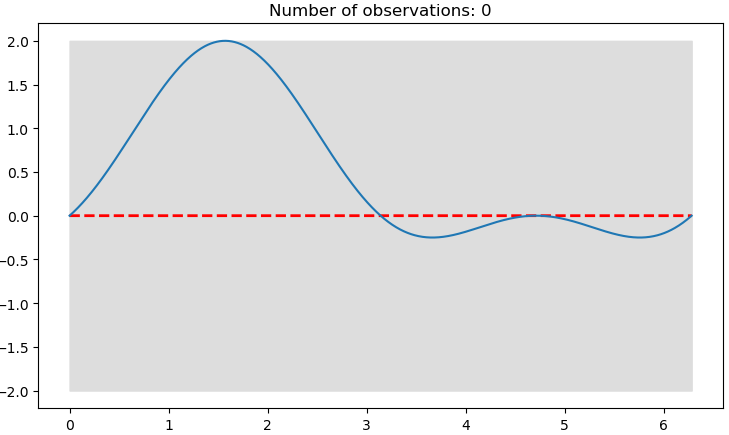
\includegraphics[width=0.6\linewidth]{pictures/GP_plot_1.png}
	\centering
	\caption{Gaussian Process for the first iteration with zero observations. We assume zero mean.}
	\label{fig:GP_1}
\end{figure}

\begin{figure}[H]
	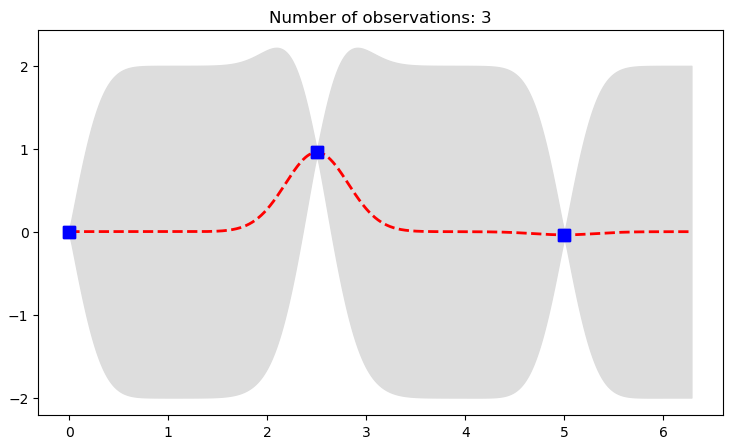
\includegraphics[width=0.6\linewidth]{pictures/GP_plot_2.png}
	\centering
	\caption{Gaussian Process for the second iteration with one observations.}
	\label{fig:GP_2}
\end{figure}

\begin{figure}[H]
	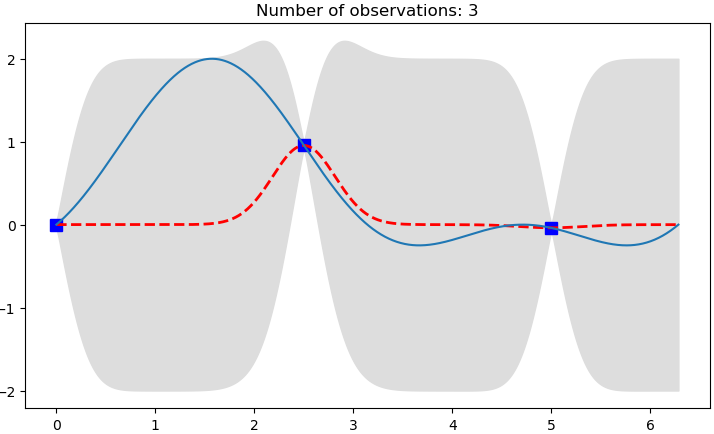
\includegraphics[width=0.6\linewidth]{pictures/GP_plot_4.png}
	\centering
	\caption{Gaussian Process for the fourth iteration with three observations.}
	\label{fig:GP_4}
\end{figure}

\begin{figure}[H]
	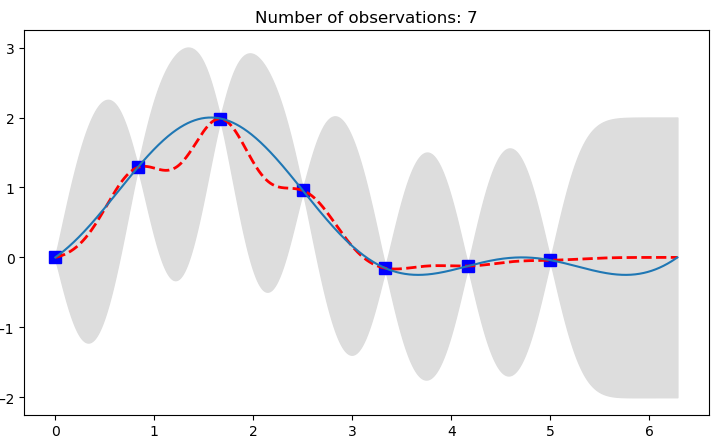
\includegraphics[width=0.6\linewidth]{pictures/GP_plot_8.png}
	\centering
	\caption{Gaussian Process for the eight iteration with seven observations.}
	\label{fig:GP_8}
\end{figure}

\begin{figure}[H]
	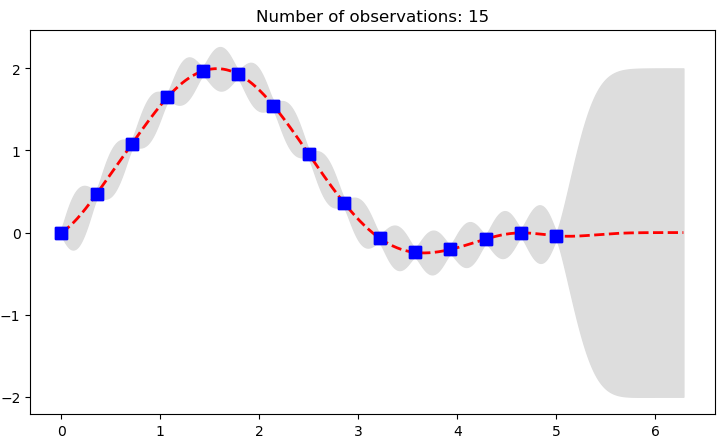
\includegraphics[width=0.6\linewidth]{pictures/GP_plot_16.png}
	\centering
	\caption{Gaussian Process for the sixteenth iteration with fifteen observations.}
	\label{fig:GP_16}
\end{figure}

\lstinputlisting[language=Python]{code/gp.py}
\end{question}

%----------------------------------------------

\end{questions}


\end{document}
